% Options for packages loaded elsewhere
\PassOptionsToPackage{unicode}{hyperref}
\PassOptionsToPackage{hyphens}{url}
%
\documentclass[
  12pt,
]{article}
\usepackage{lmodern}
\usepackage{amssymb,amsmath}
\usepackage{ifxetex,ifluatex}
\ifnum 0\ifxetex 1\fi\ifluatex 1\fi=0 % if pdftex
  \usepackage[T1]{fontenc}
  \usepackage[utf8]{inputenc}
  \usepackage{textcomp} % provide euro and other symbols
\else % if luatex or xetex
  \usepackage{unicode-math}
  \defaultfontfeatures{Scale=MatchLowercase}
  \defaultfontfeatures[\rmfamily]{Ligatures=TeX,Scale=1}
\fi
% Use upquote if available, for straight quotes in verbatim environments
\IfFileExists{upquote.sty}{\usepackage{upquote}}{}
\IfFileExists{microtype.sty}{% use microtype if available
  \usepackage[]{microtype}
  \UseMicrotypeSet[protrusion]{basicmath} % disable protrusion for tt fonts
}{}
\makeatletter
\@ifundefined{KOMAClassName}{% if non-KOMA class
  \IfFileExists{parskip.sty}{%
    \usepackage{parskip}
  }{% else
    \setlength{\parindent}{0pt}
    \setlength{\parskip}{6pt plus 2pt minus 1pt}}
}{% if KOMA class
  \KOMAoptions{parskip=half}}
\makeatother
\usepackage{xcolor}
\IfFileExists{xurl.sty}{\usepackage{xurl}}{} % add URL line breaks if available
\IfFileExists{bookmark.sty}{\usepackage{bookmark}}{\usepackage{hyperref}}
\hypersetup{
  pdftitle={Manuscript},
  pdfauthor={Nicole Schrad},
  hidelinks,
  pdfcreator={LaTeX via pandoc}}
\urlstyle{same} % disable monospaced font for URLs
\usepackage[margin = 1in]{geometry}
\usepackage{graphicx,grffile}
\makeatletter
\def\maxwidth{\ifdim\Gin@nat@width>\linewidth\linewidth\else\Gin@nat@width\fi}
\def\maxheight{\ifdim\Gin@nat@height>\textheight\textheight\else\Gin@nat@height\fi}
\makeatother
% Scale images if necessary, so that they will not overflow the page
% margins by default, and it is still possible to overwrite the defaults
% using explicit options in \includegraphics[width, height, ...]{}
\setkeys{Gin}{width=\maxwidth,height=\maxheight,keepaspectratio}
% Set default figure placement to htbp
\makeatletter
\def\fps@figure{htbp}
\makeatother
\setlength{\emergencystretch}{3em} % prevent overfull lines
\providecommand{\tightlist}{%
  \setlength{\itemsep}{0pt}\setlength{\parskip}{0pt}}
\setcounter{secnumdepth}{-\maxdimen} % remove section numbering
-\usepackages(helvet) -\renewcommand+\familydefault{\sfdefault}

\title{Manuscript}
\author{Nicole Schrad}
\date{}

\begin{document}
\maketitle

\#\#Abstract

\hypertarget{introduction}{%
\subsection{Introduction}\label{introduction}}

*Microbial metabolism drives the geochemistry, and therefore the water
quality, of aquifers. The fate of many pollutants is determined by the
pH, oxygen concentration, organic carbon availability, and the
mineralogy of the soil and infiltrating water through the unsaturated
zone.

*One such method is MAR. Managed aquifer recharge (MAR) is a set of
tools and techniques that purposefully replenishes aquifers for
environmental benefit or later recovery. There are many forms and water
sources for MAR, including diverted slope runoff, treated stormwater, or
river water.

*The objectives of this study were to (1) understand the impact of
stormwater infiltration on the soil microbial community and its
biogeochemical functioning and (2) document common changes to the
community introduced by the addition of a carbon rich PRB. We
hypothesize that that.\\
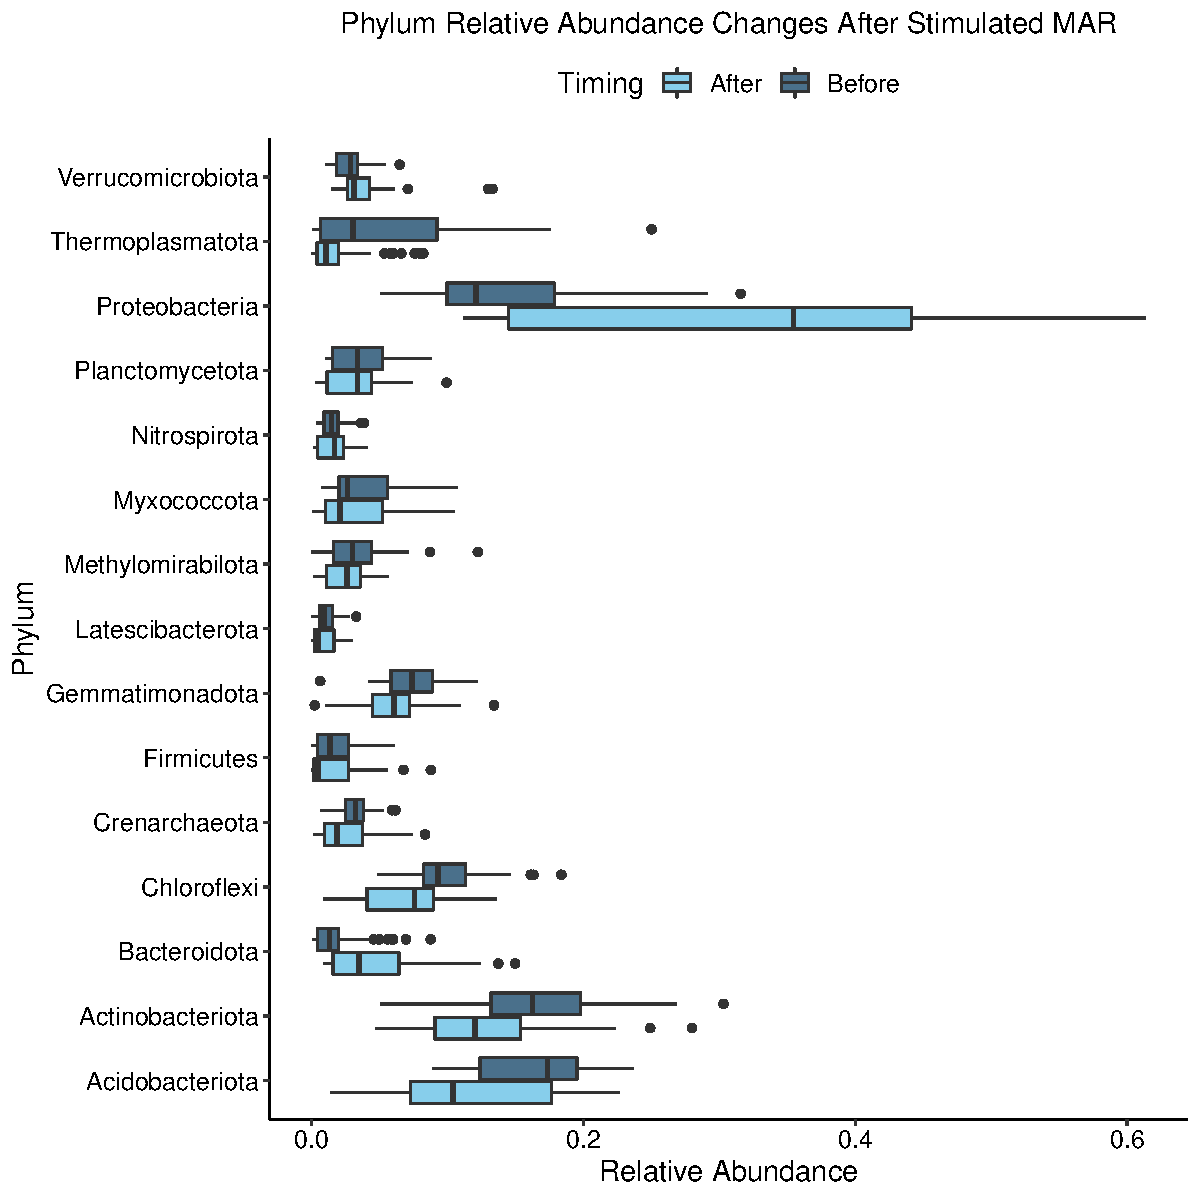
\includegraphics{Figures/unnamed-chunk-2-1.pdf}

\hypertarget{materials-and-methods}{%
\subsection{Materials and Methods}\label{materials-and-methods}}

\hypertarget{site-locations}{%
\subsubsection{Site Locations}\label{site-locations}}

\emph{3 different study locations in Pajaro Valley have 3 different soil
properties } At all locations multiple 1m \#\#\# DNA and 16S Sequencing

\hypertarget{section}{%
\subsubsection{}\label{section}}

\end{document}
